\documentclass{article}
\usepackage{assumptionsofphysics}
\usepackage{graphicx}
\graphicspath{{images/}}
\usepackage{tikz}
\usetikzlibrary{shapes,backgrounds}
\begin{document}
\title{DrawingFigs}


Work on basics of tikz package

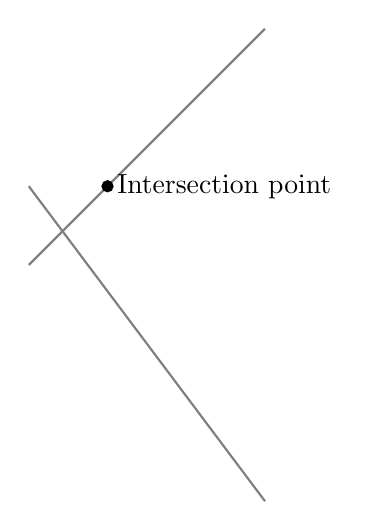
\begin{tikzpicture}
\draw[gray, thick] (-1,0) -- (2,-4);
\draw[gray, thick] (-1,-1) -- (2,2);
\filldraw[black] (0,0) circle (2pt) node[anchor=west]{Intersection point};
\end{tikzpicture}
\newpage

\pagestyle{empty}
\def\firstcircle{(-2,0) circle (2.5cm)}
\def\secondcircle{(2,0) circle (2.5cm)}
\begin{tikzpicture}
\draw \firstcircle node[above] {$Hamiltonian Mechanics$};
\draw \secondcircle node [above] {$Newtonian Mechanics$};
%\begin{scope}
%      \clip \firstcircle;
%      \fill[r] \secondcircle;
%\end{scope}

\end{tikzpicture}



\newpage
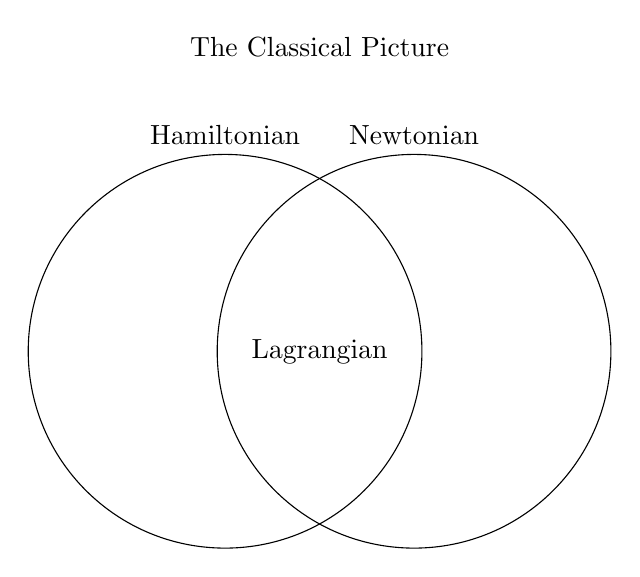
\begin{tikzpicture}
\title{The Classical Picture}

\node [label={The Classical Picture}] (C) at (1.2,3.5){};
 
% Set A
\node [draw,
    circle,
    minimum size =5cm,
    label={90:Hamiltonian}] (A) at (0,0){};
 
% Set B
\node [draw,
    circle,
    minimum size =5cm,
    label={90:Newtonian}] (B) at (2.4,0){};
 
% Set intersection label
\node at (1.2,0) {Lagrangian};
 
\end{tikzpicture}

\end{document}
